%!TEX root=./report.tex
\section{INTRODUCTION}
Research in robotics and computer vision has long considered the use of 3-D point clouds as a rich source of information about the world.
Throughout the history of research, the recognition methods and features considered have shared ideas--from early work on retrieving 3-D shape models to integrating 2-D and 3-D percepts to human pose estimation.
But the sheer diversity of applications has made it hard to see the common patterns, and nearly impossible to meaningfully compare between different choices made in the processing pipeline.

\begin{figure}[thpb]
   \centering
   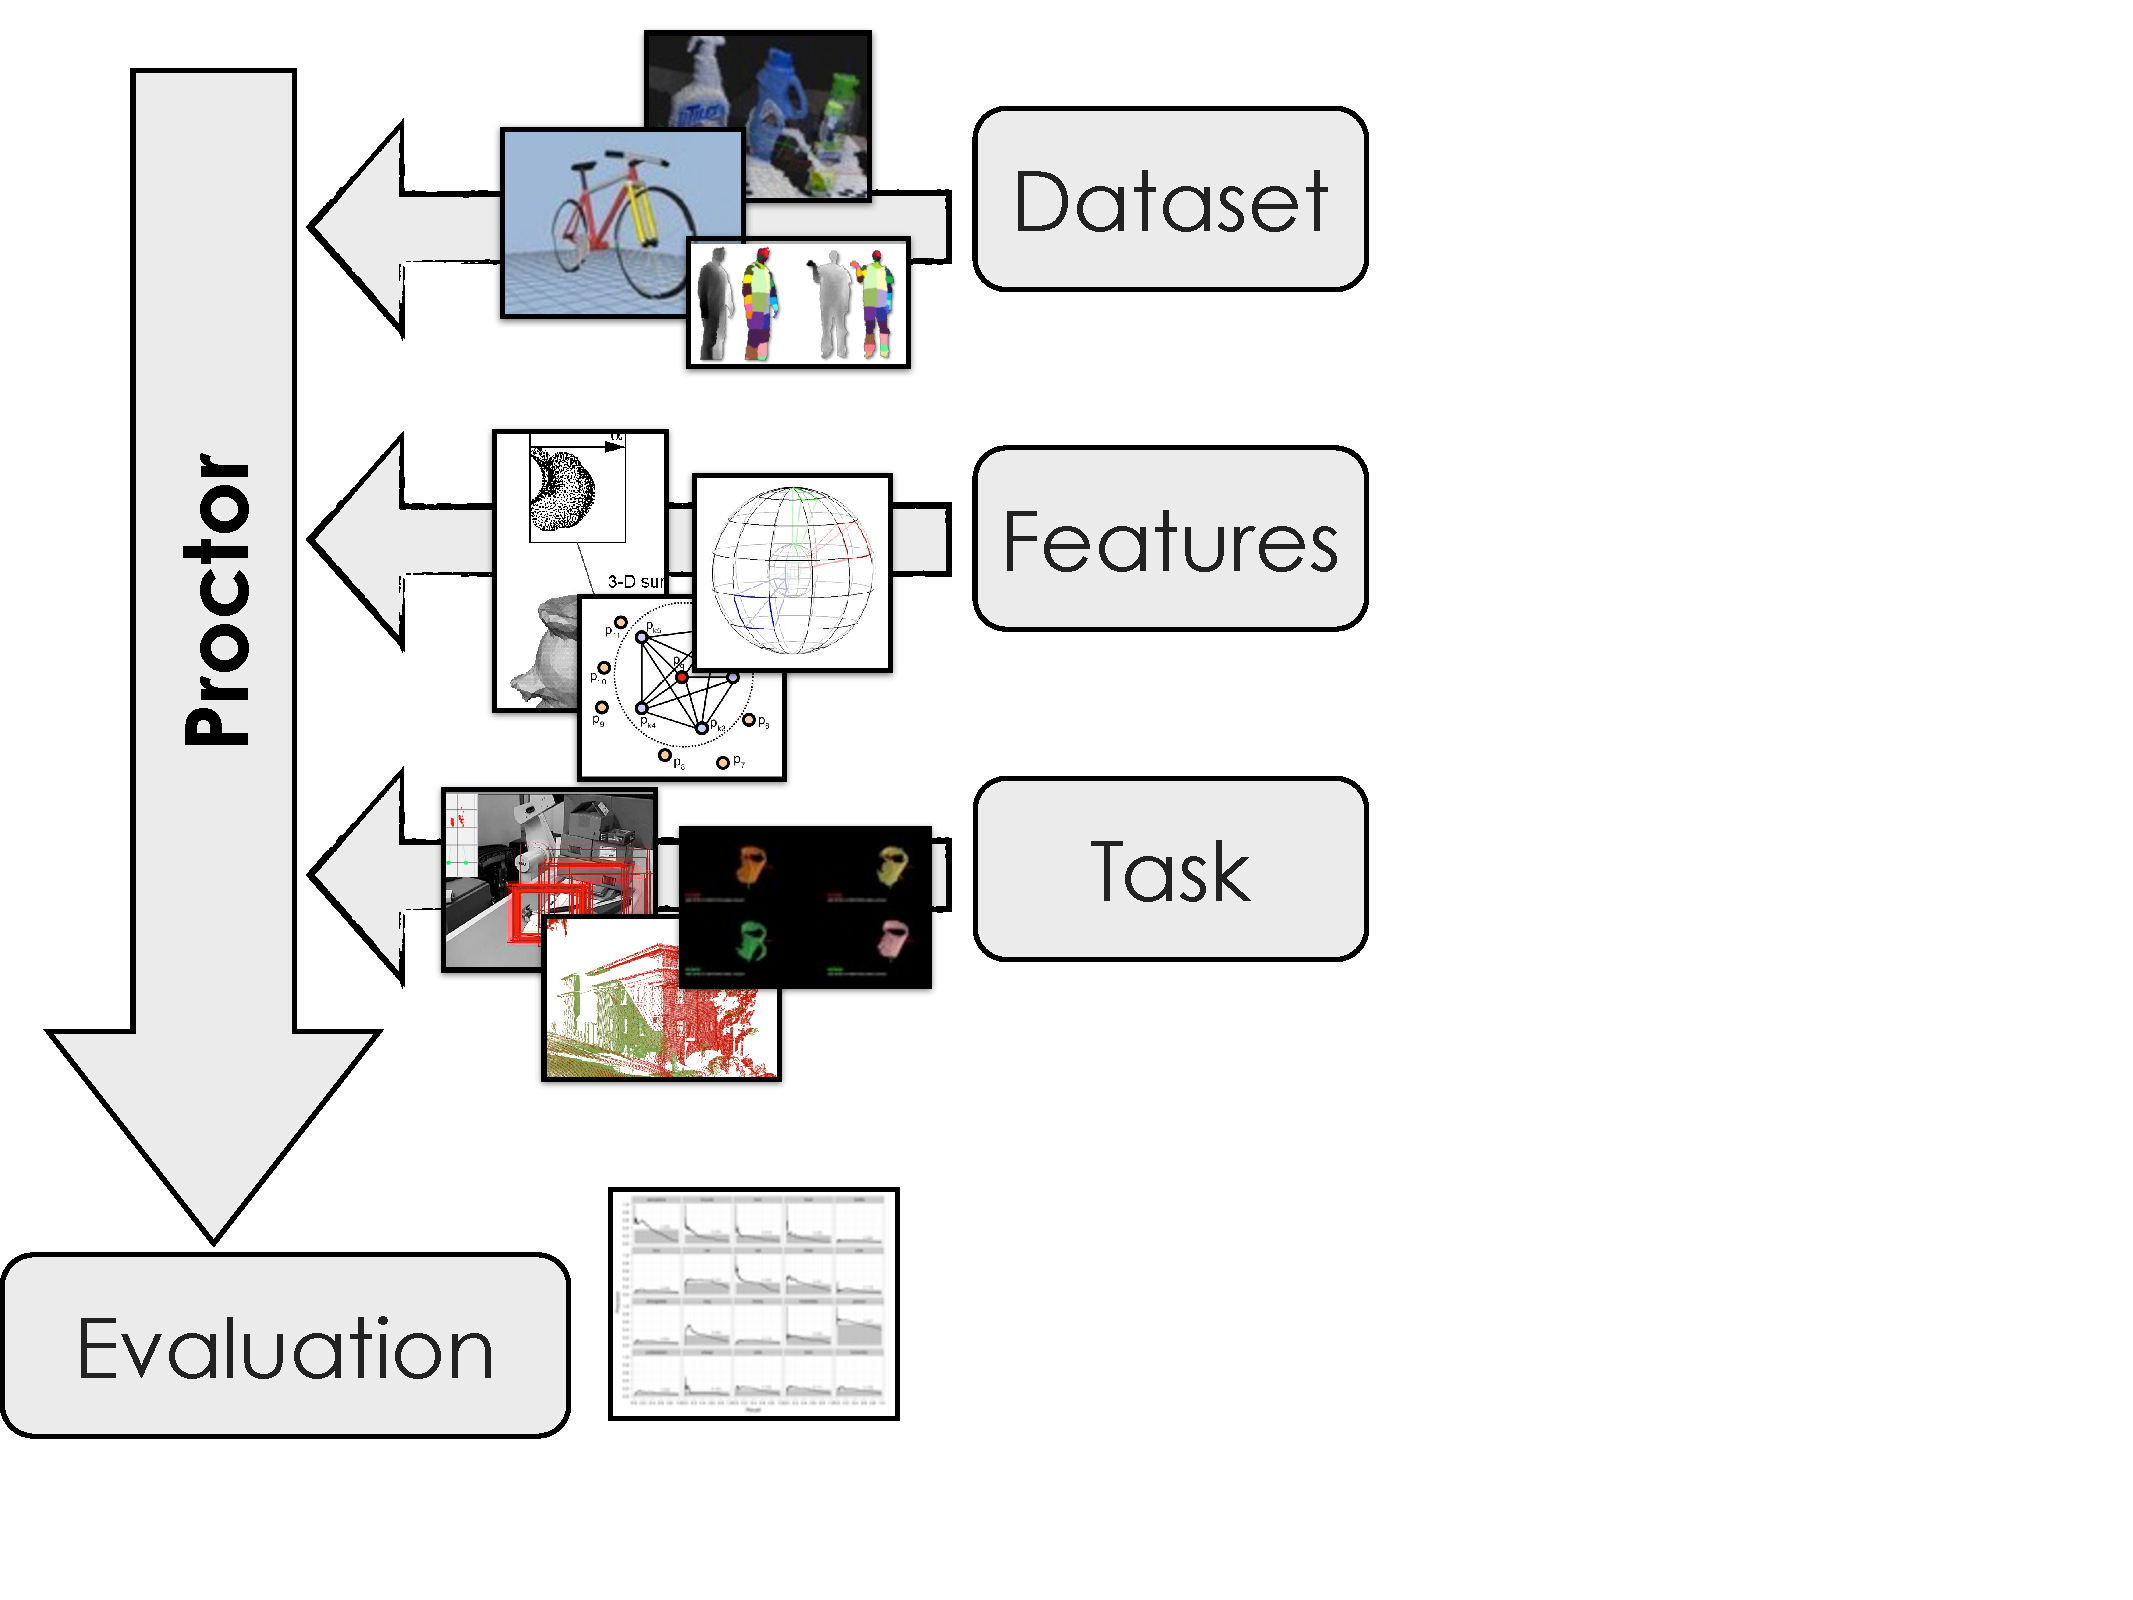
\includegraphics[width=0.45\textwidth]{figures/figure1.pdf}
   \caption{Our system modularizes the standard 3-D recognition pipeline such that individual components may be comparatively evaluated.}
   \label{fig:figure1}
\end{figure}

We hope to foster easier sharing of ideas and methods through a common evaluation framework for 3-D perception tasks.
In this paper, we present an open-source framework for comparing different 3-D features in the model matching evaluation regime.
We explain the motivations behind our system and describe its modular architecture, with the aim of encouraging a community of users and contributors.
The PR-2 \note{citation?} has facilitated rapid progress in personal robotics research due to standardization and abstraction of the hardware interface.
Our system, Proctor, aims for the same kind of impact in 3-D features, and classification and pose estimation methods research.

\section{RELATED WORK}

A full accounting of all 3-D perception tasks would not be possible given our format.
Concisely, common 3-D perception tasks can be sorted among several dimensions.

Given a database and a view, our task may be to:
\begin{itemize}
\item identify the object in the view (recognition)
\item identify the object and its pose in the view (pose estimation)
\item localize an object in the view and identify it (detection)
\end{itemize}

The view provided can be clean or cluttered.
It can be solely 3-D data, or it can include an image from a camera.
The sensor that provides the 3-D data can be LIDAR, or structured light, or a stereo camera.
It can have highly regular or random noise statistics.

Our database can consist of full polygonal models, full point cloud models, or sparse views.
In the latter cases, the models may contains noise which may or may not be of the same form as our test sensor.


\subsection{3D and 2D/3D Recognition Whirlwind Overview}
\note{sergeyk: this is lifted from B3DO paper, I am re-working and expanding this to incorporate our summer reading list}
\label{sec:2d-3d}
A comprehensive review of all 3-D features proposed for recognition is beyond the scope of our work--briefly notable prominent techniques include spin images \cite{spin}, 3-D shape context \cite{Frome3DSC}, and the recent VFH model \cite{RaduVFH}--but this list is not exhaustive. 

A number of 2D/3D hybrid approaches have been recently proposed, and our dataset should be a relevant testbed for these methods. A multi-modal object detector in which 2D and 3D are traded off in a logistic classifier is proposed by \cite{gould08eccv}. Their method leverages additional handcrafted feature derived from the 3D observation such as ``height above ground'' and ``surface normal'', which provide contextual information.
\cite{Sun2010} shows how to benefit from 3D training data in a voting based method.
Fritz et al. \cite{Fritz2010} extends branch\&bound to 3D and adds size and support surface constraints derived from the 3D observation.

Most prominently, a set of methods have been proposed for fusing 2D and 3D information for the task of pedestrian detection.
The popular HOG detector \cite{Dalal2005} to disparity-based features is extended by \cite{hattori}.
A late integration approach is proposed by \cite{rohrbach09dagm} for combining detectors on the appearance as well as depth image for pedestrian detection.
Instead of directly learning on the depth map, \cite{walk10eccv} uses a depth statistic that learns to enforce height constraints of pedestrians.
Finally, \cite{leibe10ijrr} explores pedestrian detection by using stereo and temporal information in a hough voting framework also using scene constraints.

\subsection{Features}

* Spin images \cite{Johnson1999}

* Curvature histograms, Geometric moments

* 3D Shape contexts and Harmonic shape contexts \cite{Frome2004}

* Point Feature Histograms \cite{Rusu2009}

* Andrew Ng-style combinations \cite{Gould2008,Coates2010}

* Kinect decision forest \cite{Shotton2011}

The SHREC 2011 Benchmark \cite{Boyer2011} is an evaluation of 3-D feature detection and description stages of shape retrieval algorithms.
The benchmark measures how the detection and description algorithms degrade under synthetic transformations of the 3D data, including sub-sampling, isometry, holes, shot and random noise, view, and affine.
The benchmark is inspired by similar evaluation of computer vision features(\cite{Mikolajczyk2004,Mikolajczyk2005}, and the features evaluated are largely 3-D analogs of 2-D detectors and descriptors such as the Harris corner and Difference-of-Gaussians \cite{Harris1988,Lowe2004} detectors and SIFT, HOG, and MSER descriptors \cite{Lowe2004,Dalal2005,Matas2004}.

\subsection{Datasets}
\note{some is lifted from B3DO paper}

An evaluation of a method is only as meaningful as the underlying dataset.
There are a number of available dataset for 3-D recognition, varying in size, content (3D only or with 2D views), labels (pose, instance, category, or some combination of these), and source (controlled capture or ``in the wild'').
Here we summarize the most appropriate datasets for our generalized evaluation framework.

\subsection{3D Data Only}
{\bf Princeton Shape Benchmark \cite{Shilane2004}}:
A standard evaluation for 3-D shape retrieval, classification, and clustering applications.
The models are provided in polygonal format, and are divided into standard training and test datasets.
As for many other papers in the field, this dataset provides the evaluation basis of our implementation.

\subsection{2D/3D Data}
{\bf Rgbd-dataset of \cite{Lai2011}}:
This dataset features 300 objects in 51 categories.
The category count refers to nodes in a hierarchy, with, for example, ``coffee mug'' having ``mug'' as parent.
Each category is represented by 4-6 instances, which are densely photographed on a turntable.
For object detection, only 8 short video clips are available, which lend themselves to evaluation of just 4 categories (bowl, cap, coffee mug, and soda can) and 20 instances.

{\bf UBC Visual Robot Survey \cite{Helmer2010}}:
The Visual Robot Survey dataset from UBC provides training data for 4 categories (mug, bottle, bowl, and shoe) and 30 cluttered scenes for testing detection approaches.
Each scene is photographed in a controlled setting from multiple viewpoints.

{\bf 3D table top object dataset \cite{Sun2010}}:
The ``3D table top object dataset'' covers 3 categories (mouse, mug, stapler) and provides 200 test images with cluttered background.
There is no significant viewpoint variation in the test set.

{\bf Solutions in Perception Challenge \cite{SIPC2011}}:
The dataset of the ``Solutions in Perception Challenge,'' which will take place in conjunction with ICRA'12.
The goal of the challenge is to identify the extent to which 3D recognition problem is ``solved;'' it thus focuses on the high-precision part of the performance curve.
The 2011 challenge consisted of 35 distinct objects such as branded boxes and household cleaner bottles that are presented in isolation for training and in 27 scenes for test.

{\bf A Category-level 3-D Object Dataset: Putting the Kinect to Work \cite{Janoch2011}}:
An indoor, crowd-sourced dataset collected with the Kinect sensor.
The dataset aims to capture the statistics of actual household object distribution, and to be challenging by today's standards due to large viewpoint and inter-class variation, and realistic clutter in the scenes.
The first set of results is provided on 9 object classes, but the growing nature of the dataset means that more results will be published in the future.

{\bf Other datasets:} Beyond these, a couple of other datasets have been made available which do include simultaneous capture of image and depth but serve more specialized purposes like autonomous driving \cite{ford_dataset}, pedestrian detection \cite{leibe10ijrr} and driver assistance \cite{walk10eccv}.
Their specialized nature means that they cannot be leveraged for the multi-object category localization task that is our goal.
